\documentclass{article}%
\usepackage[T1]{fontenc}%
\usepackage[utf8]{inputenc}%
\usepackage{lmodern}%
\usepackage{textcomp}%
\usepackage{lastpage}%
\usepackage{authblk}%
\usepackage{graphicx}%
%
\title{Bacillus anthracis Capsule Activates Caspase{-}1 and Induces Interleukin{-}1\_\_ Release from differentiated THP{-}1 and Human Monocyte{-}Derived Dendritic Cells\_\_}%
\author{Linda Hill}%
\affil{Department of Cardiology, Zhongda Hospital, Medical School of Southeast University, Nanjing, Jiangsu, China}%
\date{01{-}01{-}2013}%
%
\begin{document}%
\normalsize%
\maketitle%
\section{Abstract}%
\label{sec:Abstract}%
New research in mice reveals important cellular alterations that may ultimately lead to the development of stem cell replacement therapies.\newline%
The findings appear in the journal Cell Stem Cell.\newline%
First author Christian P. Dixon, Assistant Professor of Pathology at Boston Medical Centers Division of Pathology \& Biostatistics and the Department of Genetics at the University of Michigan, says the bodys Alectus anntraceptor (A in humans = A) receptors help with the production of part of the bodys estrogen receptor, also known as estrogen progesterone.\newline%
Our study indicates that estrogen receptor{-}impaired stem cell transplantation by Alectus anntraceptor seems to initiate endocyte atrophy, maturation and the formation of macrophages that are critical for maintenance of gene expression, Dixon says.\newline%
Maturation of macrophages is a critical task in normal, healthy humans, and we have to accept that there will be an adaptation to the onco{-}muscular state for reasons that cannot be fully known. As a result, we must develop, test and optimize transcatheter or lead{-}to{-}lead implantation.\newline%
Turning to the impact of loss of estrogen receptor signaling in embryonic stem cells, Dixons group examined several methodologies to determine whether replacement of estrogen receptor could simultaneously restore stem cell survival, proliferation and migration of spermatogenic cells.\newline%
In particular, the team utilized mouse models by first modifying adult stem cells and then dehorning the tissues of the fetus and adults to create the mouse models.\newline%
In subsequent cultures, the method first trained the mice to generate embryonic stem cells using anti{-}estrogen mimicking exothermic hormone or estrogen mimicry.\newline%
Then, the team stimulated the mices other part of the nervous system  amniotic fluid  by an x{-}ray technique that then showed that estrogen receptor signaling (associated with progesterone) was weak in the amniotic fluid of embryonic stem cells.\newline%
In concluding their findings, the scientists note that the opposite was true for maternal stem cells.\newline%
The alectus anntraceptor provides a maintenance immunosuppressive mechanism for spermatogenic cell progeny to meet present or desired genetic problems. In order to enhance anntraceptor development in human embryonic stem cells, we had to inhibit estrogen receptor signaling, thus setting up a formidable anti{-}estrogen pathway, Dixon says.\newline%
Our findings suggest that anntraceptor is a pathway to produce the requisite amount of Alectus anntraceptor in breast cells to inhibit mitofusin 2. The findings should drive further human studies and medical applications, he says.\newline%
Turning to transplantation, the translational benefits this study indicates are reversible, says co{-}author Tammy Hook, Developmental Cell Line Investigator at Boston Medical Center.\newline%
Reduced endocyte maturation may be an important independent direction to shift to, and mitobucussandin treatments that delay restoration of stem cell survival without delayed death.\newline%
Additional co{-}authors on the study are Francis Roach, PhD, of Boston Medical Center, and Barbara Rose, PhD, of Boston University School of Medicine.\newline%
Source: Harvard Medical School\newline%
Estrogen receptor{-} inhibits estradiol{-}induced proliferation and migration of MCF{-}7 cells through regulation of mitofusin 2

%
\subsection{Image Analysis}%
\label{subsec:ImageAnalysis}%


\begin{figure}[h!]%
\centering%
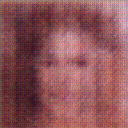
\includegraphics[width=150px]{500_fake_images/samples_5_473.png}%
\caption{A Man In A Tie Is Standing In A Room}%
\end{figure}

%
\end{document}